\section{Ejercicio 1}
\noindent
El objetivo de este ejercicio es dise\~nar la compuerta l\'ogica NOT mediante las distintas tecnolog\'ias estudiadas a lo largo del curso, es decir, \textbf{RTL} (Resistor transistor logic), \textbf{TTL} (transistor transistor logic) y \textbf{MOS}. Se busca analizar cada tecnolog\'ia para luego contrastarlas y hallar las ventajas y desventajas que presentan. 
\vspace{10mm}


{\large\textbf{Tecnolog\'ia RTL}}
\noindent
A continuaci\'on se presenta el circuito utilizado para la realizaci\'on de la compuerta NOT mediante esta tecnolog\'ia.

\begin{figure}[h!]
\center
    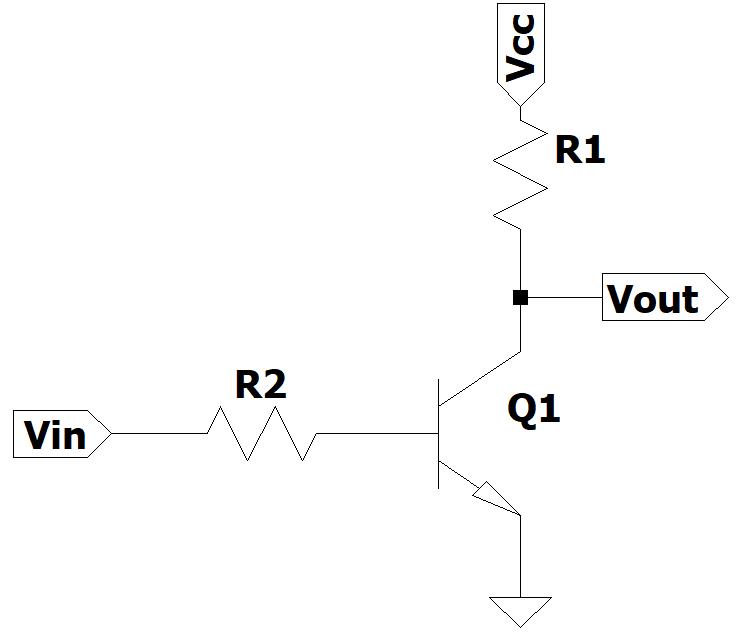
\includegraphics[scale = 0.45]{figs/ej1/not_rtl.png}
    \caption{Compuerta NOT con tecnolog\'ia RTL.}
\label{fig:ej1_rtl}
\end{figure}
\noindent
El funcionamiento de esta tecnolog\'ia se basa en que Vcc, la alimentaci\'on, se mantiene con una tensi\'on constante, por ejemplo 5V, mientras que en la entrada la tensi\'on puede variar. Si la tensi'on en la base del transistor representa un '0' l\'ogico, el transistor no conduce y por lo tanto, a la salida habr\'a un '1' l\'ogico. Por el otro lado, si se aplica un '1' l\'ogico en la base del transistor, comienza a conducir y la tensi\'on entre el colector y el emisor ser\'a de aproximadamente 0.3V representando un '0' l\'ogico.

\vspace{10mm}


{\large\textbf{Tecnolog\'ia TTL}}
\noindent
La compuerta NOT mediante tecnolog\'ia ttl funciona de la siguiente manera:

\begin{figure}[H]
\center
    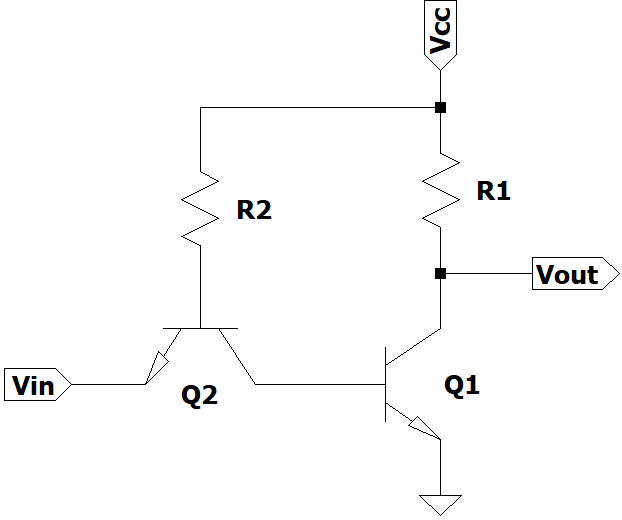
\includegraphics[scale = 0.55]{figs/ej1/not_ttl.png}
    \caption{Compuerta NOT con tecnolog\'ia TTL.}
\label{fig:ej1_ttl}
\end{figure}

\noindent\newline
El transistor Q2 trabaja tanto en directa como en inversa para dirigir la corriente hacia la base o desde la base del transistor Q1. Por lo tanto, si hay un '0' l\'ogico a la entrada Vin, con la alimentaci\'on en 5V, el transistor Q2 funciona en directa y la corriente es saliente de la base de Q1, por lo tanto, el transistor Q1 no conduce y hay un '1' a la salida. Por el contrario, si a la entrada hay un '1', el transistor Q2 est\'a polarizado en inversa y la corriente entra a la base de Q1 por lo que comienza a conducir y se ve un '0' a la salida.

\vspace{10mm}


{\large\textbf{Tecnolog\'ia MOS}}
\noindent

\begin{figure}[H]
\center
    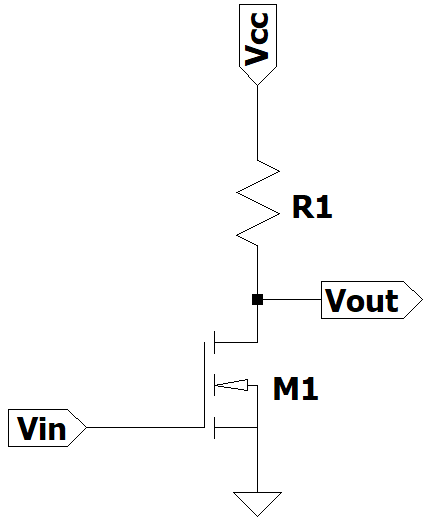
\includegraphics[scale = 0.55]{figs/ej1/not_mos.png}
    \caption{Compuerta NOT con tecnolog\'ia MOS.}
\label{fig:ej1_mos}
\end{figure}
\noindent

Se puede notar que el circuito es muy similar al rtl analizado previamente pero con un NMOS en lugar de BJT y sin la resistencia de base ya que en un MOS no circula corriente por ah\'i. Nuevamente con la tensi\'on de alimentaci\'on en 5V se analiza que pasa al aplicar a la entrada un '1' o un '0'. Si se inserta un '1', el transistor comienza a conducir y la tensi\'on entre base y emisor es de 5V por lo tanto a la salida se ve un '0'. Al insertar a la entrada un '0', el transistor no conduce y a la salida se ve un '1'.

\subsection{Mediciones}

Las mediciones se realizaron sobre un PCB que contiene las 3 compuertas juntas, como puede verse en la secci\'on \ref{ej1_pcb}.\newline
Se aliment\'o el circuito con una tensi\'on de 5V y luego, para realizar las distintas mediciones se le aplic\'o a la entrada de circuito una se\~nal cuadrada de 5V con nivel bajo en 0V para medir todo lo que est\'a relacionado con tiempos y una sen\~al tri\'angular para medir las tensi\'ones m\'inimas y m\'aximas como se detalla a continuaci\'on:\newline

\begin{itemize}
    \item VIH (\textit{High-level input voltage}): Es la m\'axima tensi\'on de entrada que el circuito interpreta como '0', produciendo un '1' a la salida. Se mide como el punto en donde la pendiente de $V_{in}(V_{out}) = -1$.
    \item VIL (\textit{Low-level input voltage}): Es la m\'inima tensi\'on de entrada que el circuito interpreta como '1', produciendo un '0' a la salida. Es el otro punto en el cual la pendiente es -1.
    \item VOH (\textit{High-level output voltage}): Es la m\'inima tensi\'on de salida con la cual hay un '1' a la salida.
    \item VOL (\textit{Low-level output voltage}): Es la m\'inima tensi\'on de salida con la cual hay un '0' a la salida.
    \item \textit{Noise margin}: Es la capacidad del circuito de tolerar ruido sin afectar el funcionamiento del mismo. Se clasifica en dos tipos:
    \begin{itemize}
        \item $NM_L$ (\textit{Low noise margin}): La diferencia entre VIL y VOL.
        \item $NM_H$ (\textit{High noise margin}): La diferencia entre VOH y VIH.
    \end{itemize}
    \item \textit{Propagation delay}: Tiempo desde que la se\~nal de entrada llega al 50\% hasta que la salida llega al mismo nivel.
    \item \textit{Transition time}: Tiempo que tarda la se\~nal de salida en llegar del 10\% hasta el 90\% de la tensi\'on al ir de '0' a '1' y viceversa para '1' a '0'.
    \item \textit{Maximum output current}: Debido a que la carga es un capacitor, se calcula como $I_c = C * \frac{dV_c}{dt}$ en donde la derivada se obtiene mediante la funci\'on \textit{math} del osciloscopio.
\end{itemize}

\begin{table}[H]
\center

\begin{tabular}{|l|c|c|c|}
\hline
\multicolumn{4}{|c|}{\textit{\textbf{Sin carga}}}                                                             \\ \hline
\multicolumn{1}{|c|}{\textbf{Tecnolog\'ia}} & \textbf{RTL} & \textbf{TTL} & \multicolumn{1}{l|}{\textbf{N-MOS}} \\ \hline
High-level input voltage.                 & 0.984V       & 0.7V         & 2.1V                                \\ \hline
Low-level input voltage.                  & 0.521V       & 0.338V       & 1.65V                               \\ \hline
High-level output voltage.                & 4.92V        & 4.998V       & 4.91V                                \\ \hline
Low-level output voltage.                 & 0.179V       & 0.096V       & 0.11V                               \\ \hline
Noise margin high.                        & 3.936V       & 4.298V       & 2.81V                               \\ \hline
Noise margin low.                         & 0.342V       & 0.242V       & 1.54V                               \\ \hline
Propagation delay high to low.            & 880ns        & 349ns        & 501ns                              \\ \hline
Propagation delay low to high.            & 29ns         & \#\#\#       & 23.95ns                              \\ \hline
Transition time high to low.              & 30.1ns       & \#\#\#         & 623ns                               \\ \hline
Transition time low to high.              & 680ns        & 382ns        & 714ns                                \\ \hline
\end{tabular}
\caption{Tabla de valores medidos sin carga.}
\label{tab:ej1_sin_carga}
\end{table}


\begin{table}[H]
\center
\begin{tabular}{|l|c|c|c|}
\hline
\multicolumn{4}{|c|}{\textit{\textbf{Con carga}}}                                                                                      \\ \hline
\multicolumn{1}{|c|}{\textbf{Tecnología}} & \textbf{RTL}              & \textbf{TTL}             & \multicolumn{1}{l|}{\textbf{N-MOS}} \\ \hline
High-level input voltage.                 & 1.02V                     & 0.822V                   & 2.15V                                \\ \hline
Low-level input voltage.                  & 0.543V                    & 0.315V                   & 1.59V                               \\ \hline
High-level output voltage.                & 4.87V                     & 4.99V                    & 4.9V                                \\ \hline
Low-level output voltage.                 & 0.247V                    & 0.067V                   & 0.18V                               \\ \hline
Noise margin high.                        & 3.85V                     & 4.168V                   & 2.75V                               \\ \hline
Noise margin low.                         & 0.296V                    & 0.248V                   & 1.41V                               \\ \hline
Propagation delay high to low.            & 8.25$\mu s$               & 7.7$\mu s$               & 6.2$\mu s$                             \\ \hline
Propagation delay low to high.            & 205$ns$                   & 46.8$ns$                 & 135$ns$                              \\ \hline
Transition time high to low.              & 146$ns$                   & 71$ns$                   & 1.12$\mu s$                               \\ \hline
Transition Time low to high.              & 25.7$\mu s$               & 21.1$\mu s$              & 23$\mu s$                                \\ \hline
Maximum output current.                   & \multicolumn{1}{l|}{11$mA$} & \multicolumn{1}{l|}{3$mA$} & \multicolumn{1}{l|}{28.2$mA$}         \\ \hline
\end{tabular}
\caption{Tabla de valores medidos con carga.}
\label{tab:ej1_con_carga}
\end{table}
\noindent
'\#\#\#' significa que dicho valor no pudo ser medido debido a las limitaciones del osciloscopio (\textit{Time rise} m\'inimo de 13ns).
\noindent\newline
\vspace{5mm}
\newline
En primer lugar, se puede observar de las mediciones hechas que el hecho de que el circuito tenga la carga de 1nF o que no lo tenga casi no afecta las tensiones de entrada ni las de salida. Mientras que por otro lado, produce que todos los tiempos, tanto de propagaci\'on como de transici\'on, aumenten, es decir, los circuitos son mas lentos con carga. \newline
Luego, se puede notar que la tecnolog\'ia TTL es la m\'as r\'apida en todos los tiempos, entre RTL y MOS, RTL es mas r\'apida en los tiempos de transici\'on pero es mas lenta en los de propagaci\'on. La gran ventaja de la tecnolog\'ia RTL es el hecho de que utiliza menos transistores que TTL. Finalmente, se puede observar que la compuerta NOT con MOS es la que presenta una mayor corriente de salida, por lo tanto es la que tiene mayor \textit{fanout}.

\subsection{Circuito utilizado}
\label{ej1_pcb}
\begin{figure}[H]
\center
    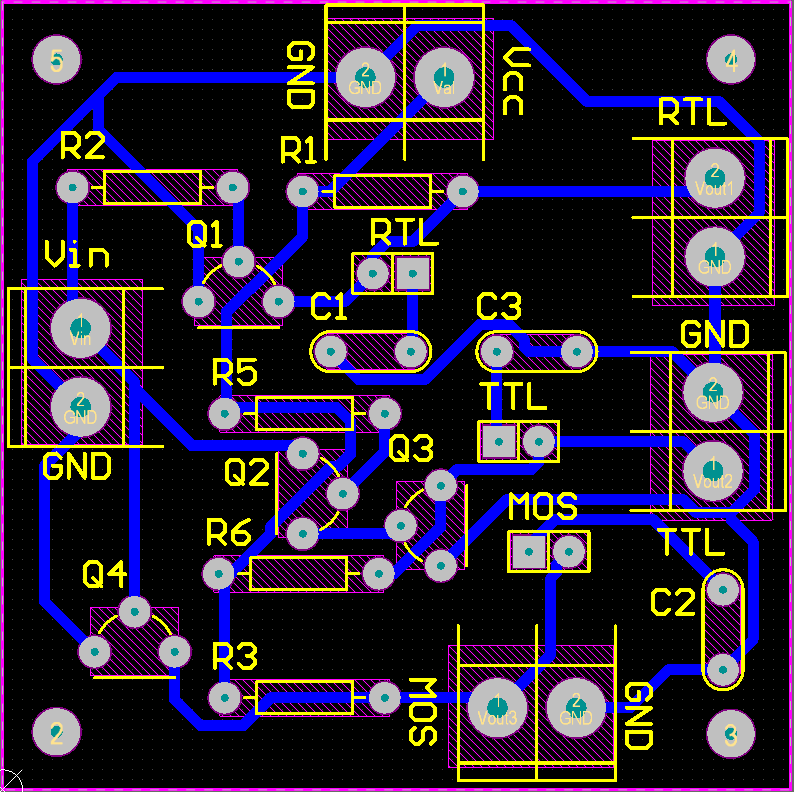
\includegraphics[scale = 0.55]{figs/ej1/ej1_PCB.png}
    \caption{Implementaci\'on del circuito en PCB.}
\label{fig:ej1_pcb}
\end{figure}
\noindent\newline